% Options for packages loaded elsewhere
\PassOptionsToPackage{unicode}{hyperref}
\PassOptionsToPackage{hyphens}{url}
%
\documentclass[
]{book}
\usepackage{amsmath,amssymb}
\usepackage{iftex}
\ifPDFTeX
  \usepackage[T1]{fontenc}
  \usepackage[utf8]{inputenc}
  \usepackage{textcomp} % provide euro and other symbols
\else % if luatex or xetex
  \usepackage{unicode-math} % this also loads fontspec
  \defaultfontfeatures{Scale=MatchLowercase}
  \defaultfontfeatures[\rmfamily]{Ligatures=TeX,Scale=1}
\fi
\usepackage{lmodern}
\ifPDFTeX\else
  % xetex/luatex font selection
\fi
% Use upquote if available, for straight quotes in verbatim environments
\IfFileExists{upquote.sty}{\usepackage{upquote}}{}
\IfFileExists{microtype.sty}{% use microtype if available
  \usepackage[]{microtype}
  \UseMicrotypeSet[protrusion]{basicmath} % disable protrusion for tt fonts
}{}
\makeatletter
\@ifundefined{KOMAClassName}{% if non-KOMA class
  \IfFileExists{parskip.sty}{%
    \usepackage{parskip}
  }{% else
    \setlength{\parindent}{0pt}
    \setlength{\parskip}{6pt plus 2pt minus 1pt}}
}{% if KOMA class
  \KOMAoptions{parskip=half}}
\makeatother
\usepackage{xcolor}
\usepackage{color}
\usepackage{fancyvrb}
\newcommand{\VerbBar}{|}
\newcommand{\VERB}{\Verb[commandchars=\\\{\}]}
\DefineVerbatimEnvironment{Highlighting}{Verbatim}{commandchars=\\\{\}}
% Add ',fontsize=\small' for more characters per line
\usepackage{framed}
\definecolor{shadecolor}{RGB}{248,248,248}
\newenvironment{Shaded}{\begin{snugshade}}{\end{snugshade}}
\newcommand{\AlertTok}[1]{\textcolor[rgb]{0.94,0.16,0.16}{#1}}
\newcommand{\AnnotationTok}[1]{\textcolor[rgb]{0.56,0.35,0.01}{\textbf{\textit{#1}}}}
\newcommand{\AttributeTok}[1]{\textcolor[rgb]{0.13,0.29,0.53}{#1}}
\newcommand{\BaseNTok}[1]{\textcolor[rgb]{0.00,0.00,0.81}{#1}}
\newcommand{\BuiltInTok}[1]{#1}
\newcommand{\CharTok}[1]{\textcolor[rgb]{0.31,0.60,0.02}{#1}}
\newcommand{\CommentTok}[1]{\textcolor[rgb]{0.56,0.35,0.01}{\textit{#1}}}
\newcommand{\CommentVarTok}[1]{\textcolor[rgb]{0.56,0.35,0.01}{\textbf{\textit{#1}}}}
\newcommand{\ConstantTok}[1]{\textcolor[rgb]{0.56,0.35,0.01}{#1}}
\newcommand{\ControlFlowTok}[1]{\textcolor[rgb]{0.13,0.29,0.53}{\textbf{#1}}}
\newcommand{\DataTypeTok}[1]{\textcolor[rgb]{0.13,0.29,0.53}{#1}}
\newcommand{\DecValTok}[1]{\textcolor[rgb]{0.00,0.00,0.81}{#1}}
\newcommand{\DocumentationTok}[1]{\textcolor[rgb]{0.56,0.35,0.01}{\textbf{\textit{#1}}}}
\newcommand{\ErrorTok}[1]{\textcolor[rgb]{0.64,0.00,0.00}{\textbf{#1}}}
\newcommand{\ExtensionTok}[1]{#1}
\newcommand{\FloatTok}[1]{\textcolor[rgb]{0.00,0.00,0.81}{#1}}
\newcommand{\FunctionTok}[1]{\textcolor[rgb]{0.13,0.29,0.53}{\textbf{#1}}}
\newcommand{\ImportTok}[1]{#1}
\newcommand{\InformationTok}[1]{\textcolor[rgb]{0.56,0.35,0.01}{\textbf{\textit{#1}}}}
\newcommand{\KeywordTok}[1]{\textcolor[rgb]{0.13,0.29,0.53}{\textbf{#1}}}
\newcommand{\NormalTok}[1]{#1}
\newcommand{\OperatorTok}[1]{\textcolor[rgb]{0.81,0.36,0.00}{\textbf{#1}}}
\newcommand{\OtherTok}[1]{\textcolor[rgb]{0.56,0.35,0.01}{#1}}
\newcommand{\PreprocessorTok}[1]{\textcolor[rgb]{0.56,0.35,0.01}{\textit{#1}}}
\newcommand{\RegionMarkerTok}[1]{#1}
\newcommand{\SpecialCharTok}[1]{\textcolor[rgb]{0.81,0.36,0.00}{\textbf{#1}}}
\newcommand{\SpecialStringTok}[1]{\textcolor[rgb]{0.31,0.60,0.02}{#1}}
\newcommand{\StringTok}[1]{\textcolor[rgb]{0.31,0.60,0.02}{#1}}
\newcommand{\VariableTok}[1]{\textcolor[rgb]{0.00,0.00,0.00}{#1}}
\newcommand{\VerbatimStringTok}[1]{\textcolor[rgb]{0.31,0.60,0.02}{#1}}
\newcommand{\WarningTok}[1]{\textcolor[rgb]{0.56,0.35,0.01}{\textbf{\textit{#1}}}}
\usepackage{longtable,booktabs,array}
\usepackage{calc} % for calculating minipage widths
% Correct order of tables after \paragraph or \subparagraph
\usepackage{etoolbox}
\makeatletter
\patchcmd\longtable{\par}{\if@noskipsec\mbox{}\fi\par}{}{}
\makeatother
% Allow footnotes in longtable head/foot
\IfFileExists{footnotehyper.sty}{\usepackage{footnotehyper}}{\usepackage{footnote}}
\makesavenoteenv{longtable}
\usepackage{graphicx}
\makeatletter
\newsavebox\pandoc@box
\newcommand*\pandocbounded[1]{% scales image to fit in text height/width
  \sbox\pandoc@box{#1}%
  \Gscale@div\@tempa{\textheight}{\dimexpr\ht\pandoc@box+\dp\pandoc@box\relax}%
  \Gscale@div\@tempb{\linewidth}{\wd\pandoc@box}%
  \ifdim\@tempb\p@<\@tempa\p@\let\@tempa\@tempb\fi% select the smaller of both
  \ifdim\@tempa\p@<\p@\scalebox{\@tempa}{\usebox\pandoc@box}%
  \else\usebox{\pandoc@box}%
  \fi%
}
% Set default figure placement to htbp
\def\fps@figure{htbp}
\makeatother
\setlength{\emergencystretch}{3em} % prevent overfull lines
\providecommand{\tightlist}{%
  \setlength{\itemsep}{0pt}\setlength{\parskip}{0pt}}
\setcounter{secnumdepth}{5}
\usepackage{booktabs}
\usepackage{amsthm}
\makeatletter
\def\thm@space@setup{%
  \thm@preskip=8pt plus 2pt minus 4pt
  \thm@postskip=\thm@preskip
}
\makeatother
\usepackage[]{natbib}
\bibliographystyle{apalike}
\usepackage{bookmark}
\IfFileExists{xurl.sty}{\usepackage{xurl}}{} % add URL line breaks if available
\urlstyle{same}
\hypersetup{
  pdftitle={Análisis de Series de Tiempo de Precios de Acciones},
  pdfauthor={Julian Rojas y Natalia Tangarife},
  hidelinks,
  pdfcreator={LaTeX via pandoc}}

\title{Análisis de Series de Tiempo de Precios de Acciones}
\author{Julian Rojas y Natalia Tangarife}
\date{2025-10-13}

\begin{document}
\maketitle

{
\setcounter{tocdepth}{1}
\tableofcontents
}
\chapter*{Propuesta de Análisis}\label{propuesta-de-anuxe1lisis}
\addcontentsline{toc}{chapter}{Propuesta de Análisis}

\section{Información a Utilizar}\label{informaciuxf3n-a-utilizar}

Para este curso trabajaremos con \textbf{series de tiempo de precios diarios de acciones} de seis empresas cotizadas en mercados estadounidenses, divididas en dos sectores:

\begin{itemize}
\tightlist
\item
  \textbf{Tecnología:} Apple (AAPL), Microsoft (MSFT), Tesla (TSLA)
\item
  \textbf{Farmacéuticas:} Pfizer (PFE), Moderna (MRNA), Johnson \& Johnson (JNJ)
\end{itemize}

Los datos abarcan el período \textbf{2015-2025 (10 años)}, proporcionando un total de \textbf{14,286 observaciones}. Las variables incluyen precios de cierre, apertura, máximos, mínimos y volúmenes de negociación diarios, obtenidos mediante la librería \texttt{quantmod} que accede a \textbf{Yahoo Finance}.

\subsection{Estadísticas Descriptivas del Dataset}\label{estaduxedsticas-descriptivas-del-dataset}

\label{tab:tabla-resumen}Estadísticas descriptivas de las series de tiempo analizadas

Ticker

Sector

Obs.

Inicio

Fin

Precio.Mín\ldots.

Precio.Máx\ldots.

Volatilidad\ldots.

Retorno.Total\ldots.

AAPL

Tecnología

2514

2015-10-13

2025-10-10

22.58

259.02

29.21

777.61

MSFT

Tecnología

2514

2015-10-13

2025-10-10

46.68

535.64

26.96

989.70

TSLA

Tecnología

2514

2015-10-13

2025-10-10

9.58

479.86

59.30

2728.89

PFE

Farmacéutica

2514

2015-10-13

2025-10-10

21.59

61.25

24.00

-20.81

MRNA

Farmacéutica

1720

2018-12-07

2025-10-10

12.26

484.47

72.08

44.25

JNJ

Farmacéutica

2514

2015-10-13

2025-10-10

94.53

191.08

18.40

99.81

\textbf{Tabla 1.} Resumen estadístico del dataset con 6 activos y 14,286 observaciones totales. Tesla presenta el mayor retorno (+2,728\%) y Moderna la mayor volatilidad (72\%).

Este período incluye cuatro fases claramente diferenciadas:

\begin{itemize}
\tightlist
\item
  \textbf{Pre-COVID (2015-2019):} Período de crecimiento estable y expansión económica
\item
  \textbf{Crisis COVID-19 (2020):} Caída abrupta del mercado y alta volatilidad
\item
  \textbf{Período de Vacunas (2021):} Desarrollo y distribución de vacunas COVID-19
\item
  \textbf{Post-pandemia (2022-2025):} Nuevas dinámicas de mercado
\end{itemize}

\subsection{Comparación por Sector}\label{comparaciuxf3n-por-sector}

\begin{figure}
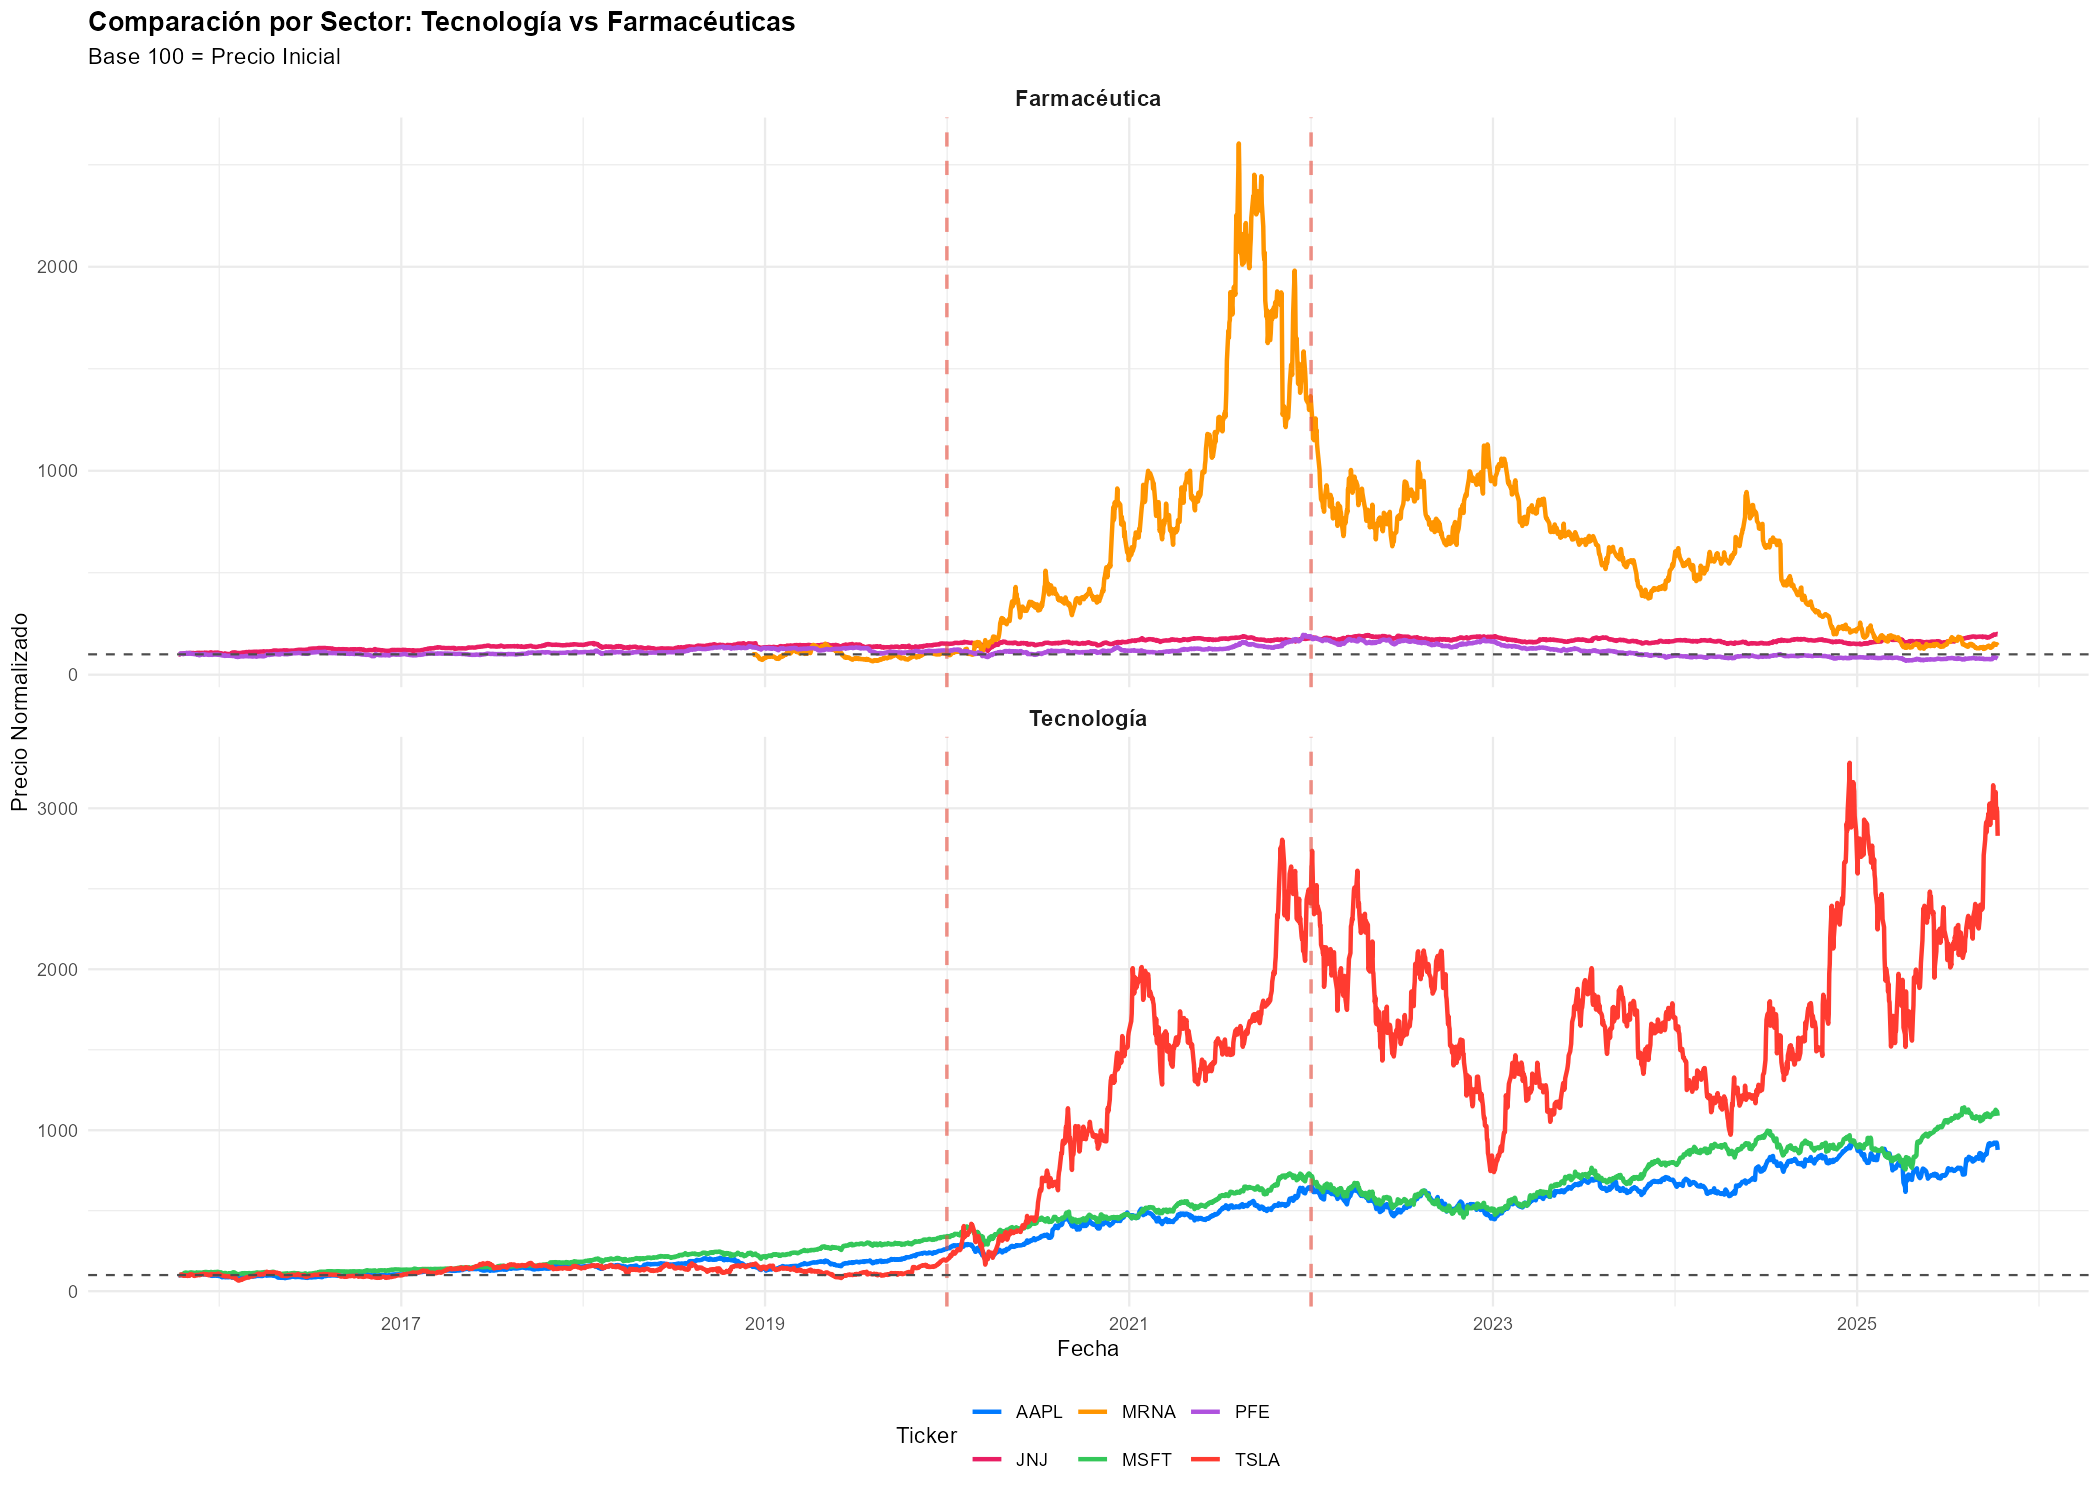
\includegraphics[width=1\linewidth]{graficos/03_comparacion_sector} \caption{Comparación de desempeño normalizado por sector. Panel superior: Farmacéuticas con Moderna mostrando crecimiento explosivo durante vacunas. Panel inferior: Tecnología con Tesla liderando los retornos. Líneas rojas verticales marcan el período COVID-19.}\label{fig:figura-sectores}
\end{figure}

La Figura 1 muestra el comportamiento diferenciado entre sectores. El sector tecnológico presenta crecimiento sostenido con Tesla liderando (+2,728\%), mientras que el farmacéutico muestra un pico en Moderna durante vacunas seguido de corrección. Este contraste será analizado en capítulos posteriores.

\section{Importancia del Pronóstico y Valor Agregado}\label{importancia-del-pronuxf3stico-y-valor-agregado}

\subsection{El Problema}\label{el-problema}

Los mercados financieros presentan comportamientos complejos que se intensifican durante crisis globales. El COVID-19 evidenció esto cuando los mercados experimentaron caídas abruptas, alta volatilidad y recuperaciones diferenciadas por sector. Los inversionistas y gestores de riesgo necesitan herramientas para anticipar movimientos de precios incluso en contextos de alta incertidumbre.

\subsection{El Valor Agregado}\label{el-valor-agregado}

Este proyecto analiza \textbf{series de tiempo de precios de acciones} durante un período de 10 años que incluye eventos extremos. El valor agregado reside en:

\textbf{1. Análisis con Datos Reales Abundantes:} Con 14,286 observaciones totales (2,514 por activo principal y 1,720 para MRNA), los análisis tienen suficiente poder estadístico para identificar patrones robustos, tendencias de largo plazo y quiebres estructurales.

\textbf{2. Múltiples Regímenes de Mercado:} El período analizado captura diferentes contextos de mercado, desde estabilidad pre-COVID hasta volatilidad extrema durante la pandemia (hasta 72\% anual en MRNA) y posterior normalización.

\textbf{3. Eventos Extremos Documentados:} El dataset incluye el crash de marzo 2020, el desarrollo de vacunas y la recuperación post-pandemia, permitiendo estudiar quiebres estructurales en series de tiempo y evaluar capacidad predictiva ante eventos de baja probabilidad pero alto impacto.

\textbf{4. Comparación Intersectorial Cuantificada:} Los datos revelan contrastes marcados:

\begin{itemize}
\tightlist
\item
  \textbf{Tecnología:} Retornos totales entre +777\% (AAPL) y +2,728\% (TSLA)
\item
  \textbf{Farmacéuticas:} Comportamiento heterogéneo desde -20\% (PFE) hasta +44\% (MRNA)
\item
  \textbf{Volatilidad:} Rango de 18\% (JNJ) hasta 72\% (MRNA)
\end{itemize}

\textbf{5. Caracterización Estadística:} Los datos permiten identificar propiedades como estacionariedad, autocorrelación, heterocedasticidad y cambios de régimen en volatilidad, aspectos que serán desarrollados en capítulos posteriores.

\textbf{6. Aplicación a Valoración de Opciones:} Los análisis de volatilidad histórica y comportamiento de precios se integran con el modelo Black-Scholes para mejorar la valoración de opciones financieras.

\section{Fuentes de Datos y Permisos de Uso}\label{fuentes-de-datos-y-permisos-de-uso}

\textbf{Fuente:} Yahoo Finance a través de la librería \texttt{quantmod} en R. Es una fuente pública reconocida en el sector financiero que permite acceso a datos históricos sin restricciones para uso académico y de investigación.

\textbf{Especificaciones técnicas:}

\begin{itemize}
\tightlist
\item
  \textbf{Período:} 2015-2025 (10 años, excepto MRNA que inicia en 2018)
\item
  \textbf{Observaciones totales:} 14,286 datos distribuidos en 6 activos
\item
  \textbf{Frecuencia:} Diaria (aproximadamente 252 días de trading por año)
\item
  \textbf{Acceso:} API pública sin permisos especiales requeridos
\item
  \textbf{Rango de precios:} Desde \$9.58 (TSLA mínimo) hasta \$535.64 (MSFT máximo)
\end{itemize}

\textbf{Variables recopiladas:}

\begin{itemize}
\tightlist
\item
  Precios: Cierre, apertura, máximo, mínimo (valores diarios en USD)
\item
  Volumen de negociación diario
\item
  Variables derivadas: Retornos diarios, retornos logarítmicos, volatilidad histórica
\item
  Clasificación temporal: Períodos COVID (Pre, Pandemia, Vacunas, Post)
\end{itemize}

\section{Impacto Esperado}\label{impacto-esperado}

El análisis de series de tiempo con más de 14,000 observaciones reales beneficia a:

\textbf{Inversionistas:} Comprensión documentada de cómo diferentes sectores responden a choques sistémicos, con evidencia cuantitativa de retornos y volatilidades observados durante crisis.

\textbf{Gestores de riesgo:} Identificación de patrones de volatilidad durante eventos extremos, con datos reales que muestran variaciones desde 18\% hasta 72\% de volatilidad anualizada según el activo y el período.

\textbf{Analistas financieros:} Caracterización cuantitativa de resiliencia sectorial respaldada por datos históricos de una década, incluyendo el evento más disruptivo de los mercados financieros en la última generación.

\textbf{Traders de opciones:} Estimación mejorada de volatilidad para valoración de derivados, con datos históricos que documentan cambios de régimen en volatilidad durante diferentes fases del mercado.

\textbf{Académicos:} Evidencia empírica robusta sobre comportamiento de series financieras durante crisis globales, con suficientes observaciones para análisis estadísticamente significativos y validación de modelos de series de tiempo.

\begin{center}\rule{0.5\linewidth}{0.5pt}\end{center}

\textbf{Nota:} Este documento constituye la propuesta inicial del proyecto. Los capítulos posteriores desarrollarán en detalle el análisis exploratorio de las series, pruebas de estacionariedad, modelado de volatilidad, identificación de quiebres estructurales y su integración con modelos de valoración de opciones financieras.

\chapter{Introduction}\label{intro}

You can label chapter and section titles using \texttt{\{\#label\}} after them, e.g., we can reference Chapter \ref{intro}. If you do not manually label them, there will be automatic labels anyway, e.g., Chapter \ref{methods}.

Figures and tables with captions will be placed in \texttt{figure} and \texttt{table} environments, respectively.

\begin{Shaded}
\begin{Highlighting}[]
\FunctionTok{par}\NormalTok{(}\AttributeTok{mar =} \FunctionTok{c}\NormalTok{(}\DecValTok{4}\NormalTok{, }\DecValTok{4}\NormalTok{, .}\DecValTok{1}\NormalTok{, .}\DecValTok{1}\NormalTok{))}
\FunctionTok{plot}\NormalTok{(pressure, }\AttributeTok{type =} \StringTok{\textquotesingle{}b\textquotesingle{}}\NormalTok{, }\AttributeTok{pch =} \DecValTok{19}\NormalTok{)}
\end{Highlighting}
\end{Shaded}

\begin{figure}

{\centering 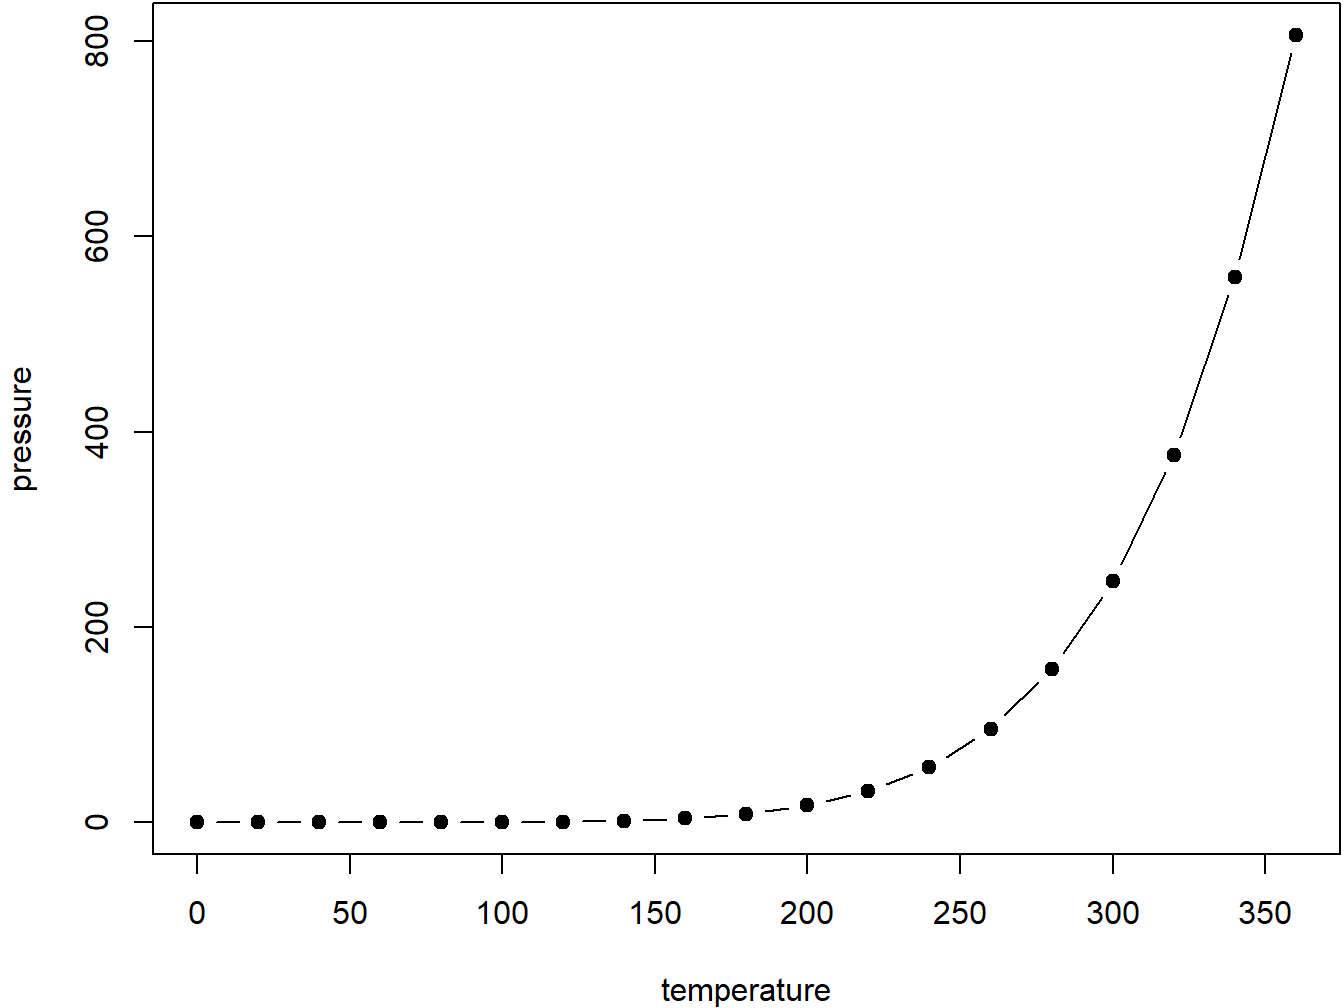
\includegraphics[width=0.8\linewidth]{01-intro_files/figure-latex/nice-fig-1} 

}

\caption{Here is a nice figure!}\label{fig:nice-fig}
\end{figure}

Reference a figure by its code chunk label with the \texttt{fig:} prefix, e.g., see Figure \ref{fig:nice-fig}. Similarly, you can reference tables generated from \texttt{knitr::kable()}, e.g., see Table \ref{tab:nice-tab}.

\begin{Shaded}
\begin{Highlighting}[]
\NormalTok{knitr}\SpecialCharTok{::}\FunctionTok{kable}\NormalTok{(}
  \FunctionTok{head}\NormalTok{(iris, }\DecValTok{20}\NormalTok{), }\AttributeTok{caption =} \StringTok{\textquotesingle{}Here is a nice table!\textquotesingle{}}\NormalTok{,}
  \AttributeTok{booktabs =} \ConstantTok{TRUE}
\NormalTok{)}
\end{Highlighting}
\end{Shaded}

\begin{table}

\caption{\label{tab:nice-tab}Here is a nice table!}
\centering
\begin{tabular}[t]{rrrrl}
\toprule
Sepal.Length & Sepal.Width & Petal.Length & Petal.Width & Species\\
\midrule
5.1 & 3.5 & 1.4 & 0.2 & setosa\\
4.9 & 3.0 & 1.4 & 0.2 & setosa\\
4.7 & 3.2 & 1.3 & 0.2 & setosa\\
4.6 & 3.1 & 1.5 & 0.2 & setosa\\
5.0 & 3.6 & 1.4 & 0.2 & setosa\\
\addlinespace
5.4 & 3.9 & 1.7 & 0.4 & setosa\\
4.6 & 3.4 & 1.4 & 0.3 & setosa\\
5.0 & 3.4 & 1.5 & 0.2 & setosa\\
4.4 & 2.9 & 1.4 & 0.2 & setosa\\
4.9 & 3.1 & 1.5 & 0.1 & setosa\\
\addlinespace
5.4 & 3.7 & 1.5 & 0.2 & setosa\\
4.8 & 3.4 & 1.6 & 0.2 & setosa\\
4.8 & 3.0 & 1.4 & 0.1 & setosa\\
4.3 & 3.0 & 1.1 & 0.1 & setosa\\
5.8 & 4.0 & 1.2 & 0.2 & setosa\\
\addlinespace
5.7 & 4.4 & 1.5 & 0.4 & setosa\\
5.4 & 3.9 & 1.3 & 0.4 & setosa\\
5.1 & 3.5 & 1.4 & 0.3 & setosa\\
5.7 & 3.8 & 1.7 & 0.3 & setosa\\
5.1 & 3.8 & 1.5 & 0.3 & setosa\\
\bottomrule
\end{tabular}
\end{table}

You can write citations, too. For example, we are using the \textbf{bookdown} package \citep{R-bookdown} in this sample book, which was built on top of R Markdown and \textbf{knitr} \citep{xie2015}.

\chapter{Literature}\label{literature}

Here is a review of existing methods.

\chapter{Methods}\label{methods}

We describe our methods in this chapter.

Math can be added in body using usual syntax like this

\section{math example}\label{math-example}

\(p\) is unknown but expected to be around 1/3. Standard error will be approximated

\[
SE = \sqrt{\frac{p(1-p)}{n}} \approx \sqrt{\frac{1/3 (1 - 1/3)} {300}} = 0.027
\]

You can also use math in footnotes like this\footnote{where we mention \(p = \frac{a}{b}\)}.

We will approximate standard error to 0.027\footnote{\(p\) is unknown but expected to be around 1/3. Standard error will be approximated

  \[
  SE = \sqrt{\frac{p(1-p)}{n}} \approx \sqrt{\frac{1/3 (1 - 1/3)} {300}} = 0.027
  \]}

\chapter{Applications}\label{applications}

Some \emph{significant} applications are demonstrated in this chapter.

\section{Example one}\label{example-one}

\section{Example two}\label{example-two}

\chapter{Final Words}\label{final-words}

We have finished a nice book.

  \bibliography{book.bib,packages.bib}

\end{document}
